%GiG
\documentclass{beamer} 
\usetheme{Copenhagen}
\setbeamertemplate{navigation symbols}{}
\setbeamertemplate{headline}{}
\DeclareMathOperator*{\argmax}{arg\,max}

\usepackage{hyperref}


\definecolor{azure}{rgb}{0.0, 0.5, 1.0}
%\newcommand{\tblue}[1]{\textcolor{blue}{#1}}
\newcommand{\tblue}[1]{{\Large {\textcolor{azure}{#1}}}}
\newcommand{\thblue}[1]{{\Huge {\textcolor{azure}{#1}}}}
\newcommand{\hred}[1]{{\textcolor{red}{#1}}}
\newcommand{\furl}[1]{{\footnote{\url{#1}}}}

\newcommand{\mypause}{\pause}
%\newcommand{\mypause}{}

\title[Saravanan Thirumuruganathan] 
{Lecture 2: Introduction To Data Visualization}

\author[CSE 5334] 
{Instructor: Saravanan Thirumuruganathan}

\date[] 

\begin{document}

\begin{frame}
  \titlepage
\end{frame}

%\begin{frame}{Outline}
%  \tableofcontents
%  % You might wish to add the option [pausesections]
%\end{frame}

\section{Outline}

\begin{frame}
\frametitle {Outline}
\begin{enumerate}
\item Data Mining Terminology
\item Basics of Visualization
    \begin{itemize}
        \item Graph integrity
        \item 2D visualization
        \item Basics of higher dimensional visualization
    \end{itemize}
\end{enumerate}
\end{frame}


\section{Announcements}
\begin{frame}{Piazza}                                                                                              
    \begin{itemize}                                                                                                          
        \item Enrollment done for registered students
        \item Auditing students - send me your email id
        \item ``Search for Teammates'' enabled
    \end{itemize}                                                                                                            
\end{frame}   

\begin{frame}{Socrative}                                                                                              
    \begin{itemize}                                                                                                          
        \item Instant Student Feedback
        \item Accessible via Smart Phone, Tablet, Laptop
        \item No login needed from Student's end
        \item Use a consistent name throughout the semester
    \end{itemize}                                                                                                            
\end{frame}   

\begin{frame}{In-Class Quizzes}
\begin{itemize}
\item {\Large {\bf URL:}} {\LARGE \bf \url{http://m.socrative.com/}} 
\item {\Large {\bf Room Name:} {\LARGE \bf 4f2bb99e}}
\end{itemize}
\end{frame}

\begin{frame}{Misc Announcements}                                                                                              
    \begin{itemize}                                                                                                          
        \item Slides for Lecture 1 updated
        \item Change Office hour timings? 
        \item Installation of Scientific Python
    \end{itemize}                                                                                                            
\end{frame}   

\begin{frame}{Other Relevant Online Classes} 
    \begin{itemize}                                                                                                          
        \item Machine Learning, Stanford: \url{https://www.coursera.org/course/ml}
        \item Mining of Massive Datasets, Stanford: \url{https://www.coursera.org/course/mmds}
        \item Statistical Learning, Stanford: \url{https://class.stanford.edu/courses/HumanitiesandScience/StatLearning/Winter2015/about}
    \end{itemize}                                                                                                            
\end{frame}   


\section{Data Mining Terminology}
\begin{frame}{}                                                                                                              
    \begin{center}                                                                                                           
        \thblue{Data Mining Terminology}                                                                         
    \end{center}                                                                                                             
\end{frame}                                                                                                                  

\begin{frame}{Data Matrix}
    \begin{center}                                                                                                           
        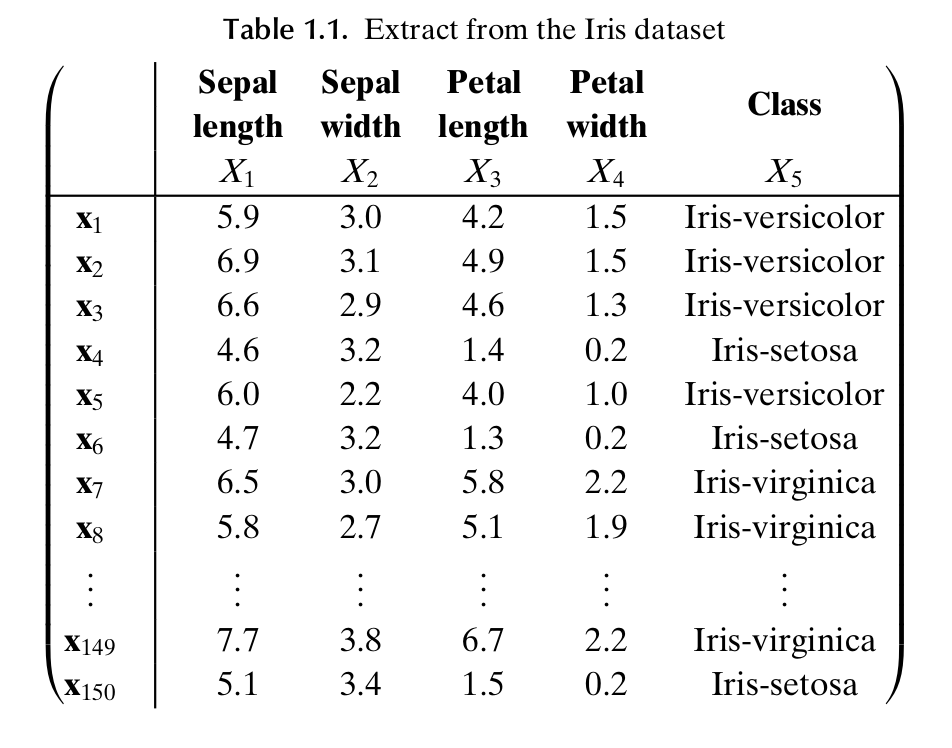
\includegraphics[scale=0.23]{dataMatrixIris.png}                                                                    
    \end{center}                                                                                                             
\end{frame}   
\begin{frame}{Data Matrix}
    \begin{center}                                                                                                           
        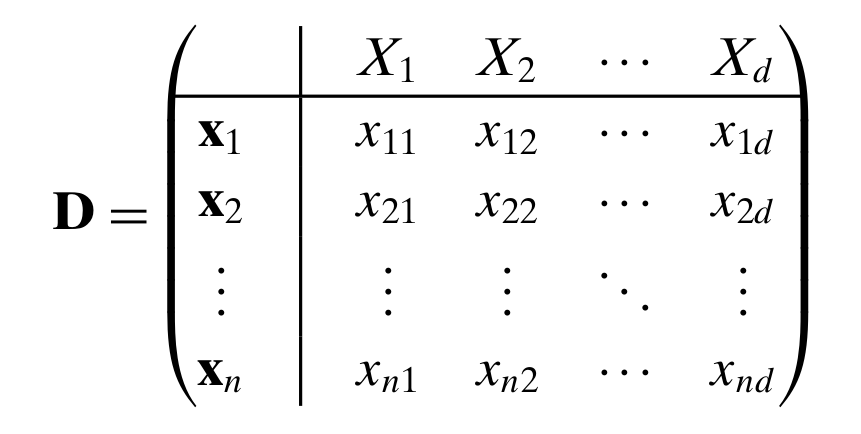
\includegraphics[scale=0.38]{dataMatrix.png}                                                                    
    \end{center}                                                                                                             
\end{frame}   


\begin{frame}{Data Matrix}                                                                                              
    \begin{itemize}                                                                                                          
        \item $n$ rows and $d$ columns 
        \item Row $\Rightarrow$ Tuple/Entities
        \item Column $\Rightarrow$ attribute/feature
        \item Special column called {\bf Class}
        \item $x_i$: $i$-th row, $X_j$: $j$-th column
        \item Row $\Rightarrow$ entities, instances, examples, records, transactions, objects, points, feature-vectors, tuples
        \item Column $\Rightarrow$ attributes, properties, features, dimensions, variables, fields
        \item $n \Rightarrow$ size, $d \Rightarrow$ dimensionality of data
    \end{itemize}                                                                                                            
\end{frame}   

\begin{frame}{Geometric View}
    \begin{center}                                                                                                           
        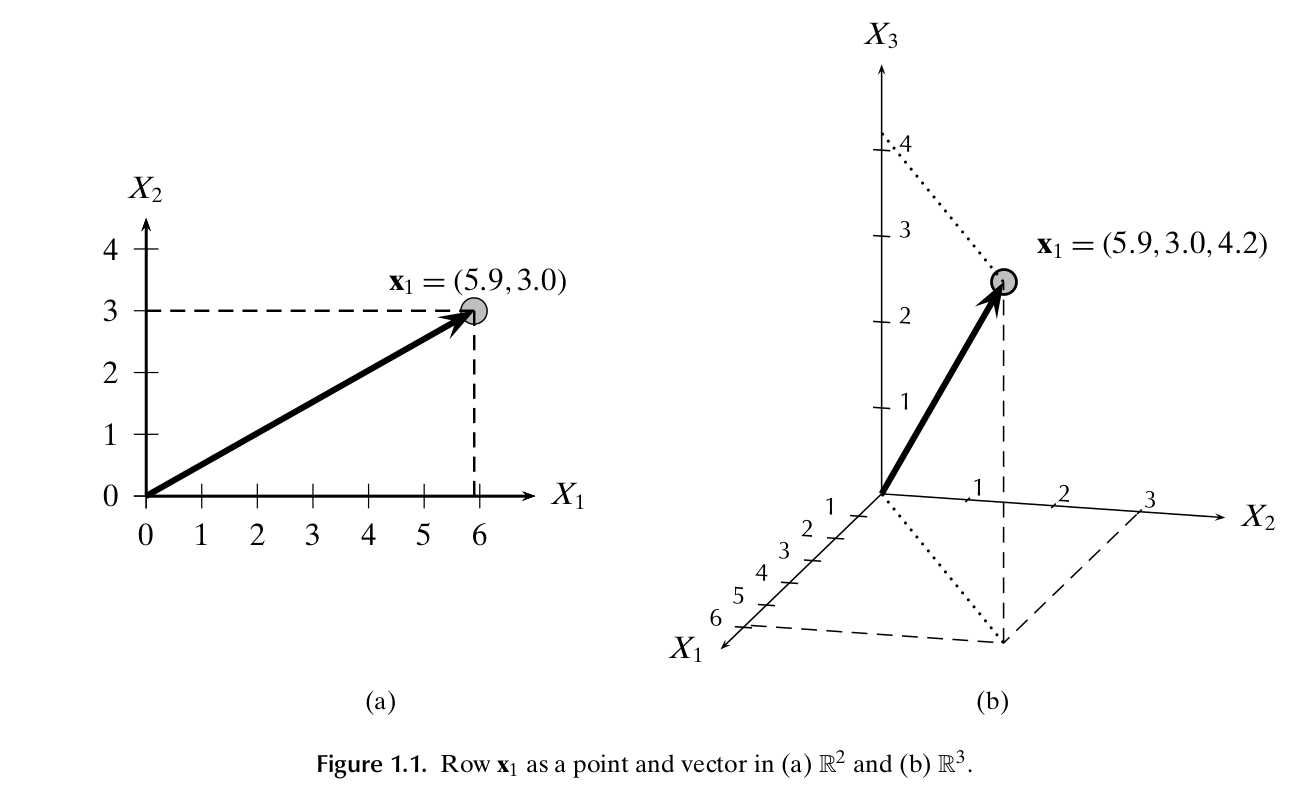
\includegraphics[scale=0.25]{geometricView.png}                                                                    
    \end{center}                                                                                                             
\end{frame}   

\begin{frame}{Implications}
    \begin{itemize}
        \item Each photo in the universe is some point in high dimension
        \item Each book (written or in future) are some point in high dimension
    \end{itemize}
    \begin{center}                                                                                                           
        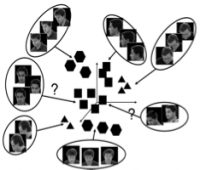
\includegraphics[scale=0.8]{faceData.png}                                                                    
    \end{center}                                                                                                             
\end{frame}   


\begin{frame}{Data Types} 

    {\bf Ben Shneiderman, 1996}:\footnote{The Eyes Have It: A Task by Data Type Taxonomy for Information Visualization [Shneiderman, 96]}
    \begin{itemize}
        \item 1D (sequences)
        \item Temporal
        \item 2D (maps)
        \item 3D (shaped)
        \item nD (relational)
        \item Trees (hierarchical)
        \item Networks (graphs)
        \item Others (text)
    \end{itemize}
\end{frame}  


\begin{frame}{Semantics vs. Types} 
    \begin{itemize}
        \item Data Semantics: real-world meaning 
        \begin{itemize}
            \item e.g., company name, day of the month, person height, etc.
        \end{itemize}
        \item Data Type: Interpretation in terms of scales of measurements
        \begin{itemize}
            \item e.g., quantity or category, sensible mathematical operations etc.
        \end{itemize}
    \end{itemize}
\end{frame}  

\begin{frame}{Data Types}
    \begin{center}                                                                                                           
        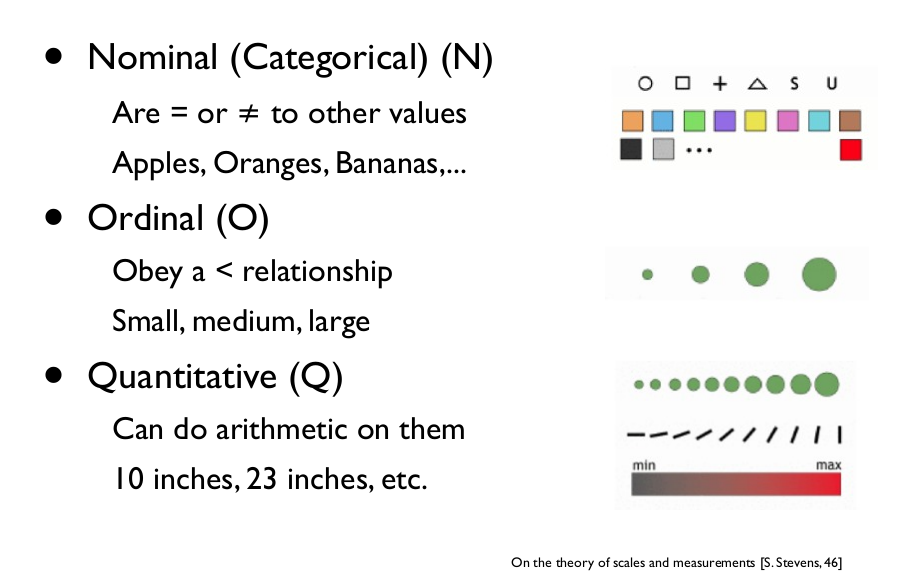
\includegraphics[scale=0.35]{dataTypes1.png}                                                                    
    \end{center}                                                                                                             
\end{frame}   

\begin{frame}{Data Types}
    \begin{center}                                                                                                           
        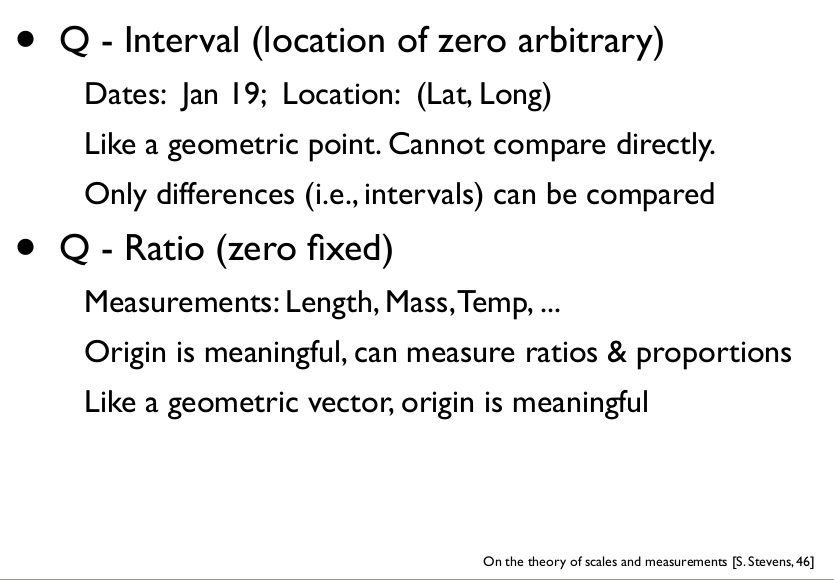
\includegraphics[scale=0.40]{dataTypes2.png}                                                
    \end{center}                                                                                                             
\end{frame}   

\begin{frame}{Data Types} 
    \begin{itemize}
        \item N - Nominal (labels) 
        \begin{itemize}
            \item Operations: \hred{$=, \neq$}
        \end{itemize}
        \item O - Ordinal (ordered)
        \begin{itemize}
            \item Operations: $=, \neq,$ \hred{$>,<$}
        \end{itemize}
        \item Q - Interval (location of zero arbitrary)
        \begin{itemize}
            \item Operations: $=, \neq, >, < $, \hred{$+,-$}
        \end{itemize}
        \item Q - Ratio (zero fixed)
        \begin{itemize}
            \item Operations: $=, \neq, >, <, +,-$, \hred{$\times, \div$}
        \end{itemize}
    \end{itemize}
\end{frame}  


\begin{frame}{Quiz!} 

    What is the data type of:
    \begin{itemize}
        \item Gender: \mypause Categorical/Nominal
        \item Age: \mypause Ordinal
        \item Height: \mypause Quantitative - Ratio 
        \item Date: \mypause Quantitative - Interval
    \end{itemize}
\end{frame}  


\begin{frame}{Data Dimensions} 
    \begin{itemize}
        \item Univariate (1D)
        \item Bivariate (2D)
        \item Trivariate (3D)
        \item Multivariate (nD)
    \end{itemize}
\end{frame}  

\section{Introduction To Data Visualization}
\begin{frame}{}                                                                                                              
    \begin{center}                                                                                                           
        \thblue{Introduction To Data Visualization}                                                                         
    \end{center}                                                                                                             
\end{frame}                                                                                                                  

\begin{frame}{Visualization Goals} 
    \begin{itemize}
        \item {\bf Presentation}
        \begin{itemize}
            \item Known facts about data
            \item Task: Communicate results
        \end{itemize}
        \item {\bf Exploration}
        \begin{itemize}
            \item Data without hypothesis   
            \item Task: Generate hypothesis
        \end{itemize}
        \item {\bf Confirmation}
        \begin{itemize}
            \item Hypothesis is given
            \item Task: Verify / falsify hypothesis
        \end{itemize}
    \end{itemize}
\end{frame}  


\begin{frame}{Visualization Goals} 
    \begin{center}
        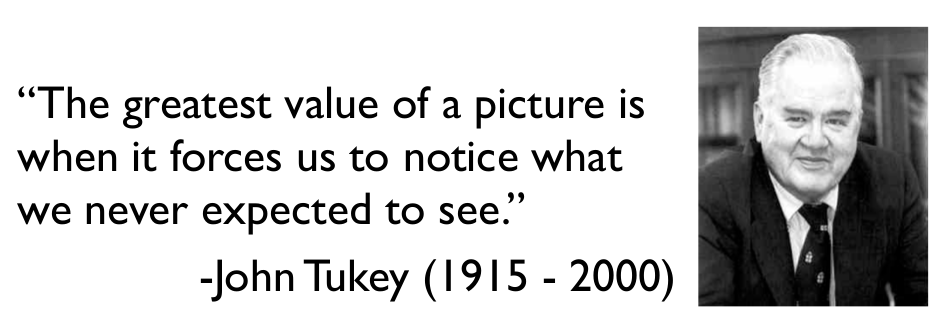
\includegraphics[scale=0.35]{tukeyEDA.png} 
    \end{center} 
\end{frame}  


\begin{frame}{Anscombe's Quartet} 

    Same mean, variance, correlation, and linear regression line
    \begin{center}                                                                                                           
        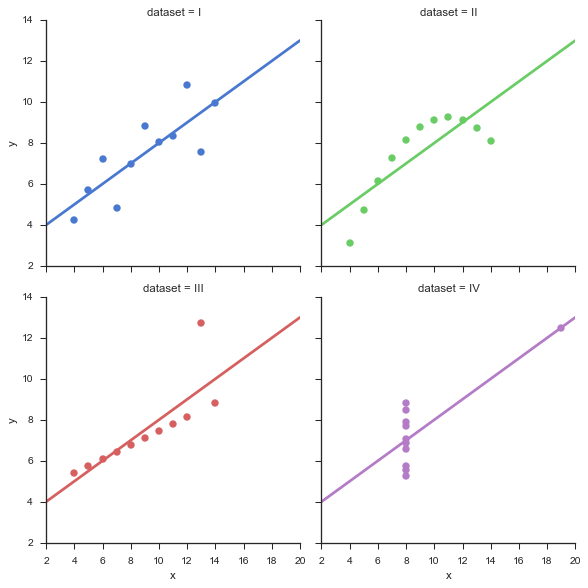
\includegraphics[scale=0.32]{anscombes_quartet.png}                                                                    
    \end{center}                                                                                                             
\end{frame}  

\begin{frame}{} 
    \begin{center}
        \thblue{Graphical Integrity}
    \end{center}
    {\bf ``There are three kinds of lies: lies, damned lies, and statistics.''} \\
    \qquad \qquad - attributed to Benjamin Disraeli in 19th Century
\end{frame}
%%%%%%%%%%%%%%%%%%%%%add graphical integrity slides here
%%%%%%%%%%%%%%%%%%%%%%%%%%%%%%%%%%%%%%%%%%%%%%%%%%%%%%%%

\begin{frame}{Labelling Chart Axes}
    \begin{center}
        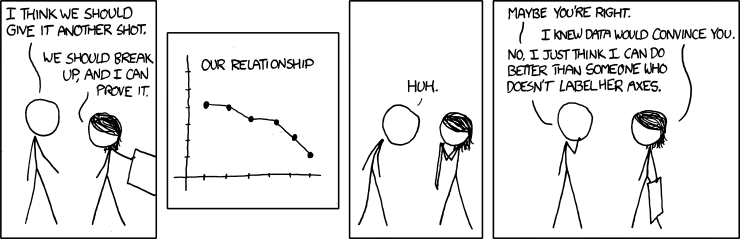
\includegraphics[scale=0.44]{xkcdConvincing.png}\furl{http://xkcd.com/833/}
    \end{center} 
\end{frame}


\begin{frame}{Lying with Scales}
    \begin{center}
        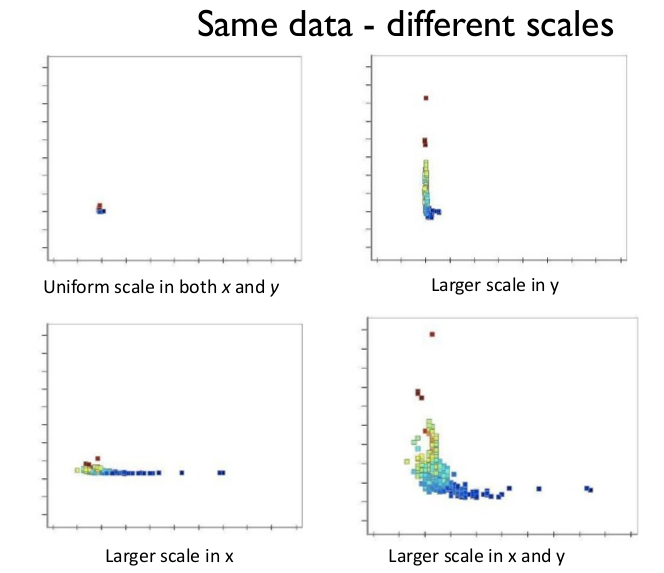
\includegraphics[scale=0.34]{lyingWithScales.png}\furl{Ward,Grinstein,Keim, 2011}
    \end{center} 
\end{frame}

\begin{frame}{Scales are Critical!} 
    \begin{itemize}
        \item What are your bounds – upper and lower?
        \item What scale works? - Linear? Log? Clipping? Breaks?    
        \item Relative or absolute values?
        \item How can you make things comparable?   
    \end{itemize}
\end{frame}  


\begin{frame}{Log Scale}
    \begin{center}
        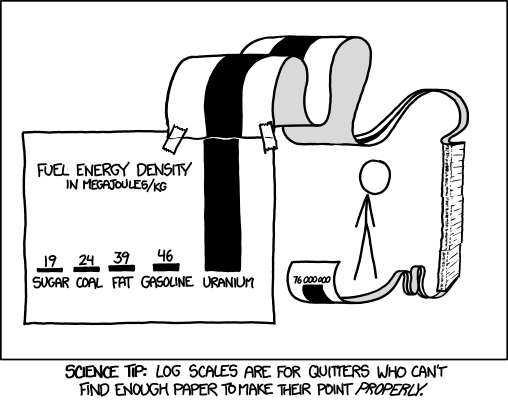
\includegraphics[scale=0.38]{xkcdLogScale.png}\furl{http://xkcd.com/1162/}
    \end{center} 
\end{frame}


\begin{frame}{} 
    \begin{center}
        \thblue{Graph Types (2D and nD)} \\
    \end{center}
\end{frame}




\section{Summary}

\begin{frame}{Summary}

\tblue{Major Concepts:}
\begin{itemize}
    \item Data mining Terminology
    \item Visualization basics
    \item Graphical Integrity
    \item Graph Types for 2D and nD
\end{itemize}
\end{frame}

\begin{frame}{Slide Material References}

\begin{itemize}
    \item Slides from Harvard CS 109 (2013 and 2014)
\end{itemize}
\end{frame}


\end{document}

